% Derivation of the Ideal Diode Equation
Consider a semiconductor material with a concentration of $n$ electrons and $p$ holes. These carrier concentrations come from two sources. The system is said to be in thermal equilibrium when no energy flows to different parts of the system or outside the system [\ref{ref:thermal_eq}]. At the thermal equilibrium, the carrier concentrations are $n_0$ and $p_0$.
Some carriers result from the system not being in thermal equilibrium. For instance, a light source may transfer energy to the material. In this case, the energy in the form of photons can excite electrons from the valence band to the conduction band, thereby producing a carrier concentration. These are known as excess carrier concentrations and are denoted by $\delta n$ and $\delta p$. Because the generation mechanisms, the excess carrier currents, etc. can be position and time dependent, these are functions of time $t$ and position $x$ in general for the one-dimensional case.
It is important to note the difference between thermal equilibrium and steady state. The generation mechanism can continually be supplying energy and producing a carrier concentration. After a while, the system reaches a steady state in which the carrier concentration no longer changes with time. However, the system is not in thermal equilibrium because it is receiving energy from the generation mechanism, such as light.
The total carrier concentrations are given by:

\begin{equation}
	\label{eq:carrier_conc}
	\begin{cases}
		n = n_0 + \delta n(x,t) \\
		p = p_0 + \delta p(x,t) \\
	\end{cases}
\end{equation}

The excess carrier concentrations depend on a few dynamics. The first is a generation process. Assume that whatever generation process exists is uniformly distributed over the material and generates at a constant rate of $g [\frac{cm^{-3}}{s}]$. When the electrons are promoted to the conduction band, they only last for as long as they have energy greater than the minimum energy of the conduction band $E_c$. Any energy they possess above $E_c$ is simply kinetic energy. The electrons move around and lose energy to collisions and other mechanisms. At a certain point, their kinetic energy is depleted, and they no longer have energy in excess of $E_c$. At this point, they fall back down to the valence band.
From this physical description, it is clear that the lifetime of these excess carriers is finite. Thus, a recombination mechanism whereby electrons fall back down to the valence band and recombine with their respective holes must be considered. This consideration is based more on physical intuition than mathematical formalisms for the sake of brevity. Essentially, the mechanism must decrease $\frac{\partial \delta n}{\partial t}$ and make it more negative since excess carriers are being depleted. With more carriers in the conduction band, more collisions between carriers occur. When they lose energy and fall down to lower and lower energy levels in the conduction band, many of them are already full, forcing them to drop all the way down to the valence band. Thus, with more carriers, this recombination mechanism must become stronger. The simplest formulation of a semiconductor with both generation and recombination mechanisms is the following:

\begin{equation}
	\label{eq:gen_and_rec}
	\frac{\partial \delta n}{\partial t} = g - \frac{\delta n}{\tau _n}
\end{equation}

Here, $\tau _n$ is the lifetime of electrons in the conduction band. When to consider electrons or holes for these calculations is discussed later.
Excess carriers are subject to drift and diffusion mechanics, causing spatial variations in the excess carrier concentration. The drift current density $J_{n,drift}$ for conduction electrons under the influence of an electric field $E$ is given by:

\begin{equation}
	\label{eq:drift}
	J_{n,drift} = qn\mu _nE
\end{equation}

Here, $q$ is the elementary charge, and $\mu _n$ is the electron mobility. Diffusion current density results from spatial variation in the carrier concentration, causing carriers to move from regions of high concentration to low concentration. The diffusion current density is given by:

\begin{equation}
	\label{eq:diffusion}
	J_{n,diff} = qD\frac{\partial \delta n}{\partial x}
\end{equation}

Including both of these effects into the current model yields the continuity equation [\ref{ref:carrier_conc_src},\ref{ref:class_slideshow}]:

\begin{align*}
	\frac{\partial \delta n}{\partial t} = \frac{1}{q} \frac{\partial J}{\partial x} + g - \frac{\delta n}{\tau _n} \\
					     = \frac{1}{q} \frac{\partial}{\partial x} ( J_{n,diff} + J_{n,drift}) + g - \frac{\delta n}{\tau _n} \\
					     = \frac{1}{q} \frac{\partial}{\partial x} ( qD\frac{\partial \delta n}{\partial x} + qn\mu _nE ) + g - \frac{\delta n}{\tau _n}
\end{align*}
\begin{equation}
	\label{eq:cont_eqn}
	\rightarrow \frac{\partial \delta n}{\partial t} = \mu _n E \frac{\partial \delta n}{\partial x} + \mu _n n \frac{\partial \delta E}{\partial x} + D_n \frac{\partial^2 \delta n}{\partial x^2} + g - \frac{\delta n}{\tau _n}
\end{equation}

A diagram of a pn-junction diode model is shown below. Essentially, the left portion is an n-type semiconductor, the right a p-type semiconductor, and the middle region is known as the space charge region.

\begin{tikzpicture}
	\label{tikz:pn-junction}
	% Horizontal line
	\draw (0.5,0) -- (9.5,0);
	% -chi n
	\draw (2,0.06) -- (2,-0.06);
	\node[ label=above:{$-\chi_{n}$} ] at (2,0) {};
	% chi p
	\draw (8,0.06) -- (8,-0.06);
	\node[ label=above:{$\chi_{p}$} ] at (8,0) {};
	% n-type region 
	\draw[ dashed ] (2,-3) -- (2,3);
	\node[ label=above:{n-Type Region} ] at (0.5,1.5) {};
	% p-type region 
	\draw[ dashed ] (8,-3) -- (8,3);
	\node[ label=above:{p-Type Region} ] at (10,1.5) {};
	% Space charge region
	\node[ label=above:{0} ] at (5,0) {};
	\node[ label=above:{Space Charge Region} ] at (5,1.5) {};
	\draw (5,0.06) -- (5,-0.06);
	% x-axis label
	\node[ label=right:{+x} ] at (9.5,0) {};
\end{tikzpicture}

A voltage $V$ is placed over the diode with high at the p-region and ground at the n-region. The three regions can essentially be viewed as three resistors in series with each absorbing a certain portion of the voltage drop. Assume the pn-junction diode is an infinitely long semiconductor slab. The electric field in each region is uniform, and its magnitude is given by:

\begin{equation}
	\label{eq:uniform_E}
	E = \frac{V_{region}}{L_{region}}
\end{equation}

Here, $V_{region}$ is the voltage over the region, and $L_{region}$ is the length of the region. If the diode is infinitely long (or simply long relative to the other lengths considered, such as the width of the space charge region), the electric field in the n- and p-type regions is $\vec{E} = \vec{0}$. Assume no external generation source, such as light exists. pn-junction diodes are typically packaged so that the interior semiconductor is covered. This way, no light can generate carriers, thereby disturbing the diode's electrical properties [\ref{ref:packaging_pn_diode}].
To analyze the steady state behavior of the pn-junction diode, solve equation (\ref{eq:cont_eqn}) with $g = 0$, $E = 0$, and $\frac{\partial f}{\partial t} = 0$ for all $f$. According to the theory of ambipolar transport, excess carriers in doped semiconductors typically take on the properties of the minority carrier. So, for the p-type region, $\delta n$ (which is the same as $\delta p$) is to be considered:

\begin{align*}
	\frac{\partial \delta n}{\partial t} = \mu _n E \frac{\partial \delta n}{\partial x} + \mu _n n \frac{\partial \delta E}{\partial x} + D_n \frac{\partial^2 \delta n}{\partial x^2} + g - \frac{\delta n}{\tau _n} \\
	\rightarrow D_n \frac{\partial^2 \delta n}{\partial x^2} - \frac{\delta n}{\tau _n} = 0
\end{align*}

\begin{equation}
	\label{eq:solve_cont_pn_p}
	\rightarrow \delta n_p(x) = A_1 e^{-\frac{x}{L_{n}}} + A_2 e^{\frac{x}{L_{n}}}
\end{equation}

Similarly, $\delta p$ is considered in the n-type region:

\begin{equation}
	\label{eq:solve_cont_pn_n}
	\delta p_n(x) = B_1 e^{-\frac{x}{L_{p}}} + B_2 e^{\frac{x}{L_{p}}}
\end{equation}

At neither edge ( $x \rightarrow \pm \infty$ ) should the excess carrier concentration become infinitely large. Imposing this boundary condition yields the following equations:

\begin{equation}
	\label{eq:carrier_conc}
	\begin{cases}
		\delta n_p(x) = A_1 e^{-\frac{x}{L_n}} \\
		\delta p_n(x) = B_2 e^{\frac{x}{L_p}}
	\end{cases}
\end{equation}

Applying what is known as the law of the junction, which relates the applied voltage to the excess carrier concentrations (\ref{ref:law_of_junction}), the following results for the excess carrier concentration can be ascertained:

\begin{equation}
	\label{eq:excess_conc_ideal_diode}
	\begin{cases}
		\delta n_p(x) = \frac{n_i^2}{N_A}(e^{\frac{qV}{k_BT}} - 1)e^{-\frac{x-\chi_p}{L_{p}}} \\
		\delta p_n(x) = \frac{n_i^2}{N_D}(e^{\frac{qV}{k_BT}} - 1)e^{-\frac{x+\chi_n}{L_{n}}}
	\end{cases}
\end{equation}

Assume that the space charge region is very thin in comparison to the quasineutral regions, i.e. the n-type and p-type regions. The current density $J$ through the space charge region is simply the sum of the current densities at the edges of the quasineutral regions. Thus, the current through the space-charge region of cross-sectional area A is given by:
\begin{align*}
	\label{eq:current_dens_ideal_diode}
		I = AJ = A(J_n(-\chi _n) + J_p(\chi _p)) \\
		       = A( (J_{n,drift}(-\chi _n) + J_{n,diff}(-\chi _n)) + (J_{p,drift}(\chi _p) + J_{p,diff}(\chi _p)) ) \\
		       = A( J_{n,diff}(-\chi _n) + J_{p,diff}(\chi _p) ) \ ( \ since \ \vec{E} = \vec{0} \ in \ the \ quasineutral \ regions \ ) \\
		       = A( qD_n\frac{\partial}{\partial x}(n_0 + \delta n_n) + qD_p\frac{\partial}{\partial x}(p_0 + \delta p_p)) \ ( by \ equation \ (\ref{eq:diffusion}) \\
		       = A( qD_n\frac{\partial \delta p_n}{\partial x} + qD_n\frac{\partial \delta n_p}{\partial x} ) \ ( since \ \delta n \ = \ \delta p \ ) \\
		       = I_0( e^{\frac{qV}{k_BT}} - 1 )
\end{align*}

\begin{equation}
	\label{eq:ideal_diode}
	\rightarrow I = I_0( e^{\frac{qV}{k_BT}} - 1 )
\end{equation}

Equation (\ref{eq:ideal_diode}) is known as the ideal diode equation, and $I_0$ is known as the reverse saturation current (\ref{ref:ideal_diode_src}). A typical plot of the ideal pn-junction diode's IV characteristic is shown in figure \ref{fig:pn-junction_iv}.

\FloatBarrier

\begin{figure}[h!]
	\centering
	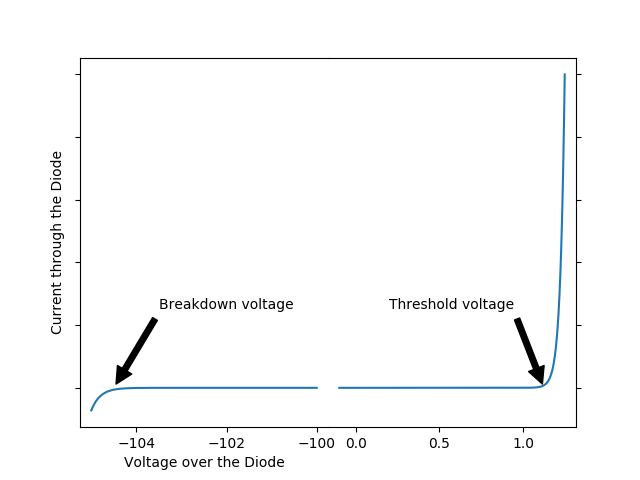
\includegraphics[scale=0.75]{../images/ideal_pn_diode.PNG}
	\caption{IV Characteristic of pn-Junction Diode}
	\label{fig:pn-junction_iv}
\end{figure}

{\footnotesize Reasonable values for plot come from source (\ref{ref:pn-plot-src}). }

\FloatBarrier

The diode is essentially off for values around 0V. This is because the electric field in the space charge region prevents any carriers from flowing. By applying a positive voltage over the diode (with the p-type region as high and the n-type region as ground), the electric field in the space charge region can be weakened, thereby allowing carriers to begin to flow. At a certain point, typically around and past the threshold voltage, the space charge region's electric field has been weakened to the point where carriers can freely flow. At a certain point, the diode essentially acts as a short circuit.
When the diode is reverse-biased, or when the polarity of the voltage source is flipped, the electric field in the space charge region is fortified, preventing charges from flowing. However, some may still leak through the diode, which gives rise to a tiny reverse saturation current. The current is essentially $-I_0$.
If the reverse-bias voltage becomes sufficiently negative, then the diode breaks down and charges are able to flow through in the opposite direction of the forward-bias case. This is typically undesired behavior in pn-junction diodes and results in a damaged diode.

\FloatBarrier

\begin{table}[h!]
	\centering
	\caption{pn-Junction Diode Results}
	\label{tab:pn-junction-results}
	\csvautotabular{../tables/pn_junction_table.csv}
\end{table}

\FloatBarrier

\begin{figure}[h!]
	\centering
	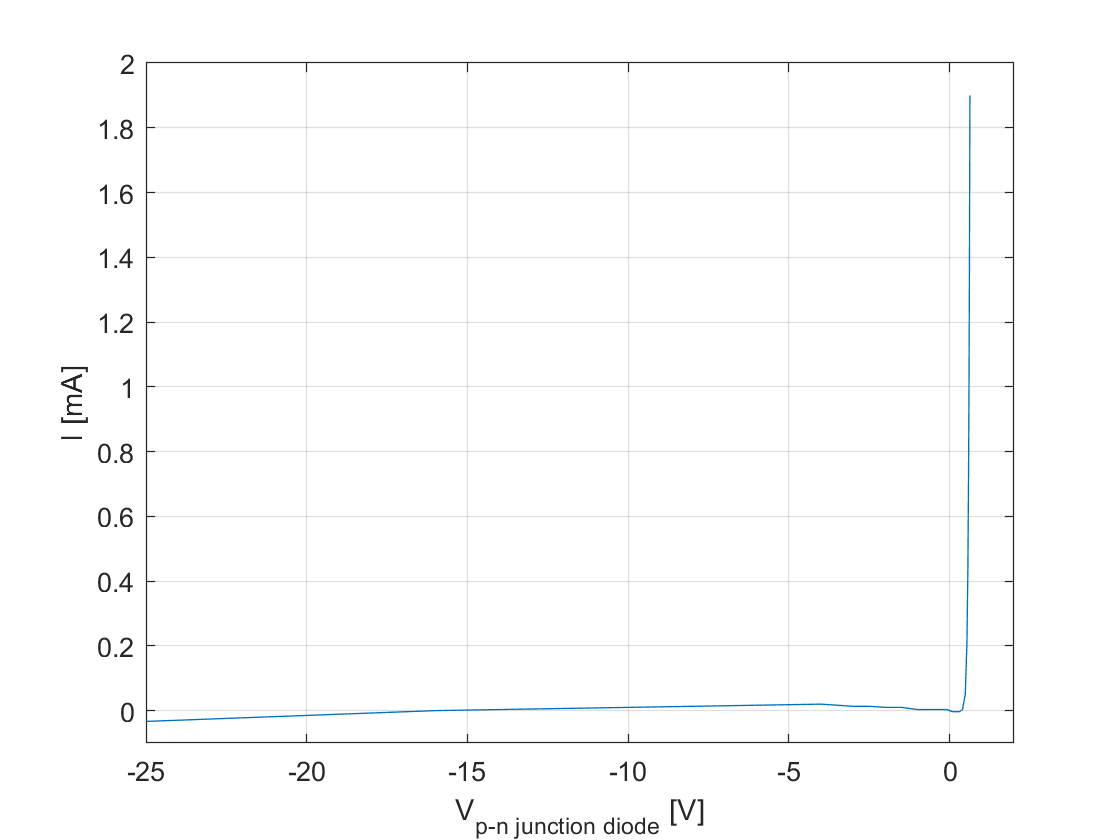
\includegraphics[scale=0.4]{../images/pn_diode.PNG}
	\caption{Measured IV Characteristic Curve of pn-Junction Diode}
	\label{fig:pn_iv_measured}
\end{figure}

\FloatBarrier

\begin{figure}[h!]
	\centering
	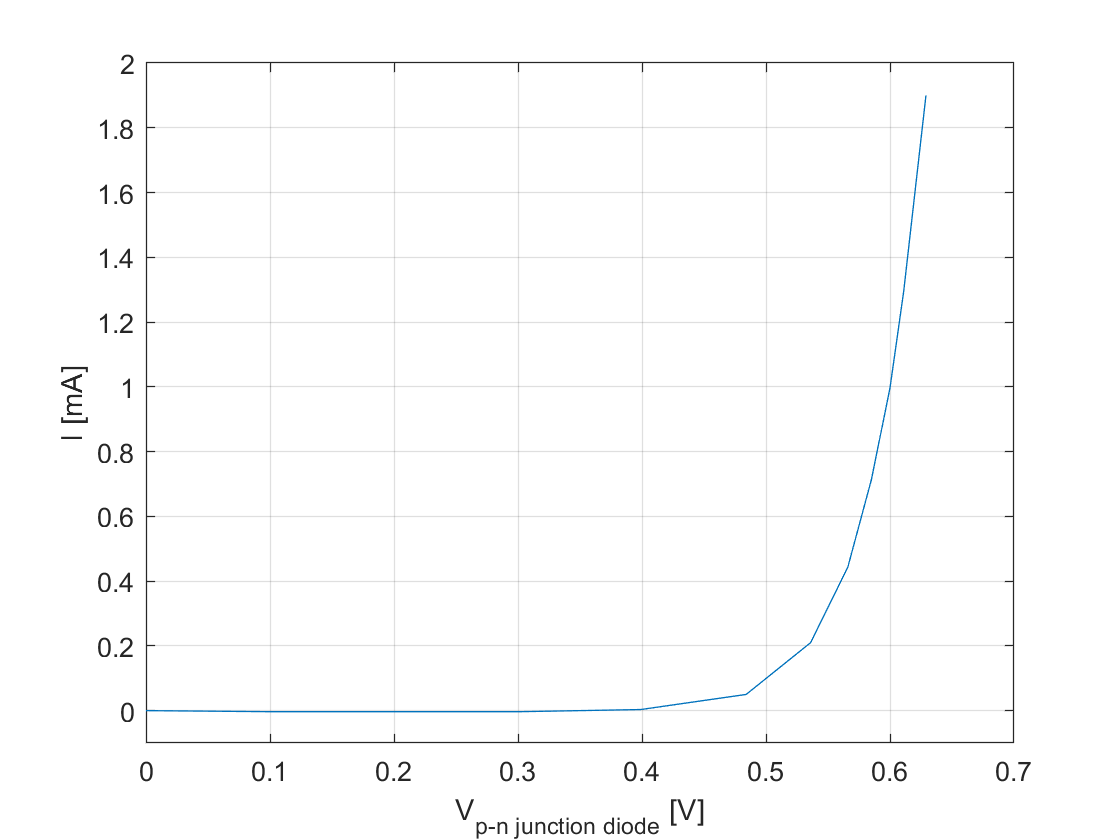
\includegraphics[scale=0.8]{../images/pn_diode_turn_on.PNG}
	\caption{Measured Turn-on Voltage of pn-Junction Diode}
	\label{fig:pn_iv_turn_on}
\end{figure}

\FloatBarrier

Taking the calculated currents and voltages over the diode from Table \ref{tab:pn-junction-results}, Figure \ref{fig:pn_iv_measured} is generated. Zooming in to the forward bias region of the curve (Figure \ref{fig:pn_iv_turn_on}), turn-on voltage is observed to be approximately $0.6 V$, which is well within typical expectation. The breakdown voltage is too large to be observed in the DC voltage sweep as no hint of breakdown is indicated by the curve in Figure \ref{fig:pn_iv_measured}, but the breakdown voltage is expected to be greater than $100 V$ (\ref{ref:pn-plot-src}).